\documentclass[14pt,a4paper]{article}
\usepackage[utf8]{inputenc}
\usepackage[russianb]{babel}
\usepackage[left=1.5cm,right=1.5cm,top=2cm,bottom=2.5cm]{geometry}
\usepackage{setspace}
\usepackage{indentfirst}
\usepackage{amssymb}
\usepackage{amsmath}
\usepackage{bm}

\usepackage{array}
\usepackage[pdftex]{graphicx}
\usepackage{comment}
\usepackage[table,xcdraw]{xcolor}


\usepackage{verbatim}


\graphicspath{{images/}}
\renewcommand{\baselinestretch}{1.3}

\begin{document}

Для начала нарисуем результат работы Черепахи, будем использовать
библиотеку turtle. Видим, что в алгоритме довольно большие числа,
поэтому увеличим размер экрана. Также зададим масштаб в переменной
scale, чтобы картинка не была слишком мелкой. На неё мы будем
умножать координаты и перемещения. Запишем алгоритм.

\begin{verbatim}
from turtle import *

# Увеличиваем размер экрана, чтобы картинка влезла
screensize(2000, 2000)

# Ускорение отрисовки
tracer(0)
# Поворот влево, чтобы Черепаха смотрел вдоль оси ординат
left(90)

# Масштаб
scale = 30

# Повтори 9
for _ in range(9):
    # Впедёд 22
    forward(22 * scale)
    # Направо 90
    right(90)
    # Вперёд 6
    forward(6 * scale)
    # Направо 90
    right(90)

# Поднять хвост
up()
# Вперёд 1
forward(1 * scale)
# Направо 90
right(90)
# Вперёд 5
forward(5 * scale)
# Налево 90
left(90)
# Опустить хвост
down()

# Повтори 9
for _ in range(9):
    # Вперёд 53
    forward(53 * scale)
    # Направо 90
    right(90)
    # Вперёд 75
    forward(75 * scale)
    # Направо 90
    right(90)


# Поднимаем хвост, чтобы нарисовать точки
up()
# Рисуем точки с координатами от -30 до 30
for x in range(-30, 30):
    for y in range(-30, 30):
        # Перемещаем Черепаху в точку (x, y)
        goto(x * scale, y * scale)
        # Зелёная точка
        dot(5, "green")


# Отрисовать рисунок
update()
# Конец программы, чтобы рисунок сразу не закрылся
done()
\end{verbatim}

Рассмотрим получившуюся картинку:

\begin{center}
    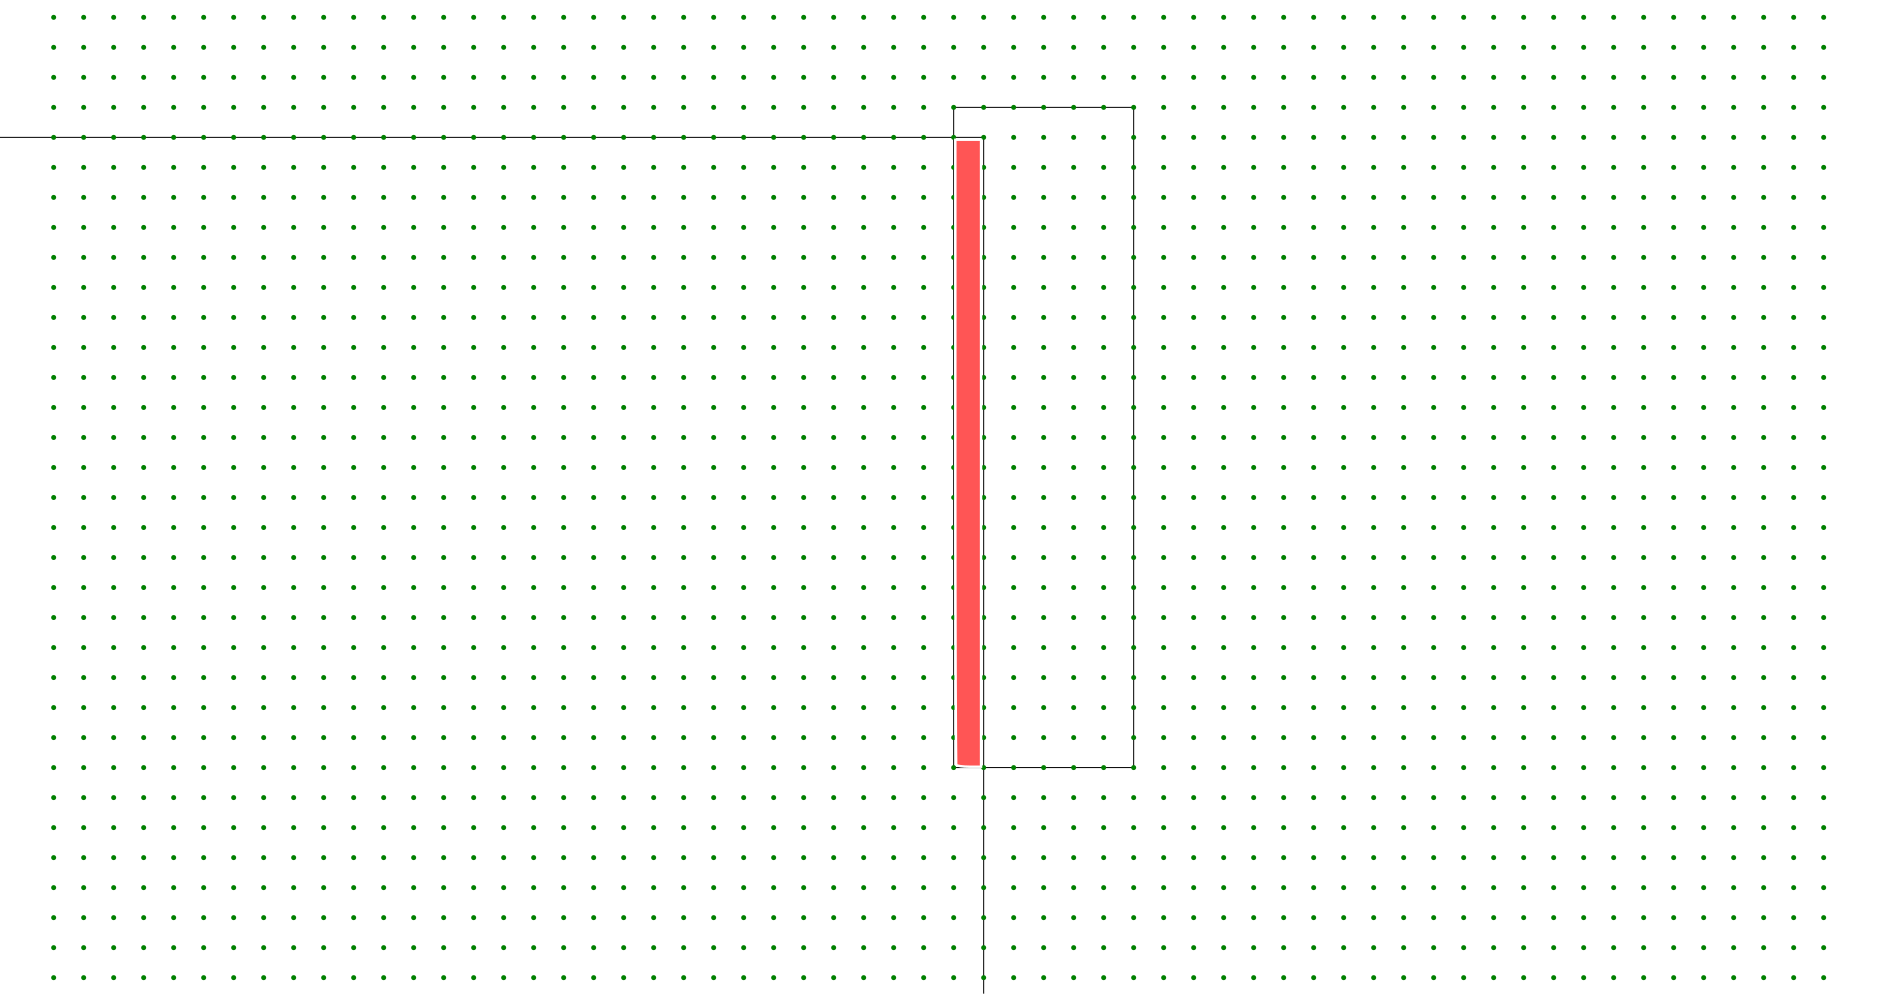
\includegraphics[width=0.5\textwidth]{figure.png}
\end{center}

Область пересечений фигур - это прямоугольник со сторонами 1 и 21.
\[\text{Периметр} = (1 + 21) \cdot 2 = 44\]

\end{document}
